%\documentclass[11pt,a4paper,twoside]{article}
\documentclass[11pt]{article}

%\usepackage[in,headings]{fullpage}
%\usepackage[french]{babel}
\usepackage[T1]{fontenc}
\usepackage{graphicx}
\usepackage{epsfig}
\usepackage{amsmath}
\usepackage{amssymb}
\usepackage{amscd}
%\usepackage{pslatex}
\usepackage{hyperref}

%\input{raccourcis}

%\newlength{\mylabelwidth}
%\settowidth{\mylabelwidth}{\labelitemi}
%\newlength{\myleftmargin}
%\setlength{\myleftmargin}{\mylabelwidth}
%\addtolength{\myleftmargin}{\labelsep}

\textwidth 16cm
\textheight 23cm
\footskip 1.5cm
\headsep 0.5cm
\oddsidemargin 0.cm
\evensidemargin 0cm
\headheight -0cm
\topmargin 0cm

\title{
	{\Large {\bf Landau damping \& Bump-on-Tail instability}} \\
	{\Large  Y. Sarazin, V. Grandgirard} \\
	{\small\it  CEA, IRFM, Saint-Paul-lez-Durance, F-13108, France} \\
	{\Large  D. Zarzoso} \\
	{\small\it  Aix-Marseille Universit\'e, CNRS PIIM, UMR 7345 Marseille, France}}

\newcommand{\dd}{\textrm d}
\newcommand{\ee}{\textrm e}
\newcommand{\Abf}{{\bf A}}
\newcommand{\Bbf}{{\bf B}}
\newcommand{\Ebf}{{\bf E}}
\newcommand{\Fbf}{{\bf F}}
\newcommand{\Jbf}{{\bf J}}
\newcommand{\Qbf}{{\bf Q}}
\newcommand{\Rbf}{{\bf R}}
\newcommand{\Sbf}{{\bf S}}
\newcommand{\Vbf}{{\bf V}}
\newcommand{\Xbf}{{\bf X}}
\newcommand{\bbf}{{\bf b}}
\newcommand{\ebf}{{\bf e}}
\newcommand{\jbf}{{\bf j}}
\newcommand{\pbf}{{\bf p}}
\newcommand{\qbf}{{\bf q}}
\newcommand{\ubf}{{\bf u}}
\newcommand{\vbf}{{\bf v}}
\newcommand{\xbf}{{\bf x}}
\newcommand{\rhobfs}{\mbox{\boldmath${\rho_s}$}}
\newcommand{\Bstar}{B_{\|}^{\ast}}
\newcommand{\vecbstar}{\mathbf b^{\ast}}
\newcommand{\vecBstar}{\mathbf B^{\ast}}
\newcommand{\vgpar}{{v_{G\parallel}}}
\newcommand{\bvgpar}{\bar v_{G\parallel}}
\newcommand{\nablabf}{{\pmb\nabla}}
\newcommand{\lhs}{left hand side }
\newcommand{\rhs}{right hand side }
\def\NN{{\rm I\hspace{-0.50ex}N} }
\def\RR{{\rm I\hspace{-0.50ex}R} }

\newcommand{\beq}{\begin{equation}}
\newcommand{\eeq}{\end{equation}}
\newcommand{\beqs}{\begin{equation*}}
\newcommand{\eeqs}{\end{equation*}}
\newcommand{\beqa}{\begin{eqnarray}}
\newcommand{\eeqa}{\end{eqnarray}}
\newcommand{\beqas}{\begin{eqnarray*}}
\newcommand{\eeqas}{\end{eqnarray*}}

\begin{document}
	\maketitle
%\today


This document discusses the physics of Landau damping and Bump-on-tail instability on the basis of a 2-dimensional kinetic model (1D-1V).
They both rely on the same equations, namely Vlasov for the electrons (ions are assumed at rest) and Poisson. The only difference comes from the equilibrium distribution function one considers, which is either a centered Maxwellian (Landau) or a centered Maxwellian with a bump on the tail (bump-on-tail). Wile the former is stable -- energy is transferred from the electrostatic wave to particles, the latter reveals unstable -- the perturbed wave grows exponentially in time in the linear regime.

%===========================================
\section{Resonance and Landau damping} \label{sec:Landau}
%===========================================
\label{s_LandauDamping}

Following the pioneering work of Landau on the subject in 1946\footnote{ L.D. Landau (1946), \emph{"On the vibrations of the electronic plasma"}, in "Collected papers of L.D.Landau", D. Ter Haar Editor, Pergamon Press, 1965, {\bf 61}, p.445}, one considers the collisionless dynamics of non relativistic electrons, embedded in a strong uniform magnetic field. The problem is assumed to be electrostatic, and the ions are at rest with a density $n_0$. The electron distribution function $f$ and the electric potential $\phi$ then compose a self consistent system governed by the Vlasov and Poisson equations:
\begin{eqnarray}\label{eq_VlasovPoisson}
  && \partial_{\tau}f + v\,\partial_{x}f +
     \partial_{x}\phi\,\partial_{v}f = 0 \\
  && \partial^{2}_{x}\phi = \int_{-\infty}^{+\infty}\!\! f \dd v -1
  \nonumber
\end{eqnarray}
Here, the radial position $r$ along the magnetic field is normalized to the Debye length $x \equiv r/\lambda_D =r/ (\varepsilon_0T/n_ee^2)^{1/2}$, time $t$ by the inverse of the electron plasma frequency $\tau\equiv \omega_{pe}t = $v$_{Te}t/\lambda_D$ and velocity by the thermal velocity v$_{Te} =(T_e/m_e)^{1/2}$: $v=$v$/$v$_{Te}$. Also, the distribution function is normalized by v$_{Te}/n_e$ ($f\rightarrow f$v$_{Te}/n_e$) and the electric potential $\Phi$ by $T_e/e$: $\phi=e\Phi/T_e$. The problem is two-dimensional in phase space $(x,v)$. We will focus on the linear characteristics of the system~\eqref{eq_VlasovPoisson}. \\

The Vlasov equation  can be rewritten in the Hamiltonian framework. Let $H$ be the dimensionless Hamiltonian of the system, sum of kinetic and potential energies:
\beq \label{eq:Hamiltonian}
H = \frac{v^2}{2} - \phi
\eeq
the minus sign coming from the electron charge. Then, eq.\eqref{eq_VlasovPoisson} can be recast as follows:
\beq \label{eq:Vlasov_Hamiltonian}
\partial_t f -\{H,f\} = 0
\eeq
with $\{H,f\}$ the Poisson brackets: $\{H,f\} = \partial_x H\partial_v f - \partial_v H\partial_x f$ (notice that it also admits the equivalent expression: $\{H,f\} = \partial_v(f\partial_x H) - \partial_x(f\partial_v H)$). $x$ and $v$ are canonically conjugated with respect to $H$:
\beqa
\dd_t x &=& \partial_v H = v \\
\dd_t v &=& -\partial_x H = \partial_x\phi
\eeqa
This formulation allows one to straightforwardly show that both the total entropy $\mathcal{S} = -\langle f\, \ln f\rangle_{x,v}$ and energy $\mathcal{E} = \frac{1}{2} \left[\langle v^2 f\rangle_{x,v} + \langle(\partial_x\phi)^2\rangle_x \right]$ are conserved, where the brackets $\langle ...\rangle_{x,v}$ stand for the integral over the entire phase space $\langle ...\rangle_{x,v} = \int\!\dd x \int\!\dd v ...$.

\noindent 
Indeed, multiplying eq.\eqref{eq:Vlasov_Hamiltonian} by $H$ and integrating over space and velocity leads to:
\beqs
\left\langle H\partial_t f \right\rangle_{x,v} 
- \frac{1}{2}\left\langle \{H^2,f\} \right\rangle_{x,v} = 0
\eeqs
Assuming periodic boundary conditions in $x$, the second term vanishes (use the second expression of the Poisson brackets). The former contains two contributions. One associated to the energy of the particles: $\frac{1}{2} \langle v^2 f\rangle_{x,v}$, the other one associated to the waves: $-\langle \phi \partial_t f\rangle_{x,v}$. Using Poisson and integrating by part, this latter term can be recast as $\langle \partial_x\phi \, \partial_t(\partial_x\phi) \rangle_x = \frac{\dd}{\dd t}  \frac{1}{2} \langle (\partial_x\phi)^2 \rangle_x$, which completes the demonstration.

\noindent 
A similar analysis can be done for the entropy. Noticing that $(f\ln f)^\prime = (1+\ln f)f^\prime$ (where the prime $^\prime$ denotes any derivative with respect to $t$, $x$ or $v$), one gets: $\frac{\dd}{\dd t}\mathcal{S} = -\langle (1+ \ln f) \{H,f\}\rangle_{x,v} = -\langle \{H,f\ln f\}\rangle_{x,v} = 0$.

%------------------------------------------------------------------
\subsection{The dispersion relation}
\label{ss_disp_relation}


Let us consider perturbations around a given stationary
equilibrium, characterized by a vanishing electric field,
$\phi_{eq}=0$. The Vlasov equation constrains the equilibrium distribution
function to depend on the velocity only: $f_{eq}(v)$. The total
distribution function $f(x,v,t)$ then takes the form: $f(x,v,t) =
f_{eq}(v) + \tilde f(x,v,t)$, with $\langle \tilde f \rangle = 0$
by definition. Here, the brackets refer to space average. \\

In the limit of small perturbations $\tilde f\ll f_{eq}$, the non
linear term can be linearized and restricted to $\partial_x
\tilde\phi \,\partial_v f_{eq}$ -- the non linearity $\partial_x
\tilde\phi \,\partial_v \tilde f$ being of the second order. At
leading order, the system~\eqref{eq_VlasovPoisson} then reduces to:
\begin{eqnarray}\label{eq_VlasovPoisson_lin}
&& \partial_{\tau}\tilde f +
  v\,\partial_{x} \tilde f +
  \partial_{x}\tilde\phi \,\partial_{v}f_{eq} = 0 \\
&& \partial^{2}_{x}\tilde \phi
   = \int_{-\infty}^{+\infty}\!\! \tilde f \dd v \nonumber
\end{eqnarray}
Consistently with the hypothesis $\phi_{eq}=0$, the electron and
ion equilibrium densities are equal to $n_0$.\\

Since the system~\eqref{eq_VlasovPoisson_lin} is linear and $f_{eq}$
depends on the velocity only, plane waves of the form
$\exp\{i(kx-\omega t)\}$ are eigenvectors 
\footnote{ 
%Rigorously speaking, plane waves are not physically acceptable solutions, since they carry infinite energy. 
Landau first introduced the concept of causality in this problem, by noticing that the waves should vanish at $t\rightarrow -\infty$. In this framework, Laplace transform in time should be preferred. However, such a change does not modify the dispersion relation. The rigorous treatment can be found, for instance, in the original paper by Landau (1946).}
. For such waves, the linearized system transforms
into:
\begin{eqnarray*}
\label{eq_VlasovPoisson_Fourier}
&& -i(\omega-kv)\hat f_{k,\omega} +
  i k\hat\phi_{k,\omega}\,\partial_v f_{eq} = 0 \\
&& -k^{2} \hat\phi_{k,\omega} =
  \int_{-\infty}^{+\infty}\!\! \hat f_{k,\omega} \dd v
\end{eqnarray*}
Combining these two equations leads to the dispersion relation:
\begin{equation}
 \label{eq_VlasovPoisson_reldisp}
  \mathcal{D} (k,\omega)= k^2 + \int_{-\infty}^{+\infty}
  \frac{k\, \partial_v f_{eq}}{\omega - kv} \dd v = 0
\end{equation}
As such, the dispersion relation remains ill posed. Indeed, the integrand contains the pole $\omega/k$ when $\omega$ is real -- corresponding to the resonant condition $\omega = kv$ from the physical point of view. So as to ensure the continuity of the integral when $\omega$ crosses the real axes\footnote{Notice that such a property is not mandatory \emph{a priori}: imposing the continuity of the integral reveals a strong assumption, with critical consequences that are detailed below.}, the integral needs being \emph{analytically continued}. Such an analytic continuation proceeds by the deformation of the integration contour into the complex plane, so as to circumscribe the pole. As detailed in Appendix \ref{Appendix_Landau}, the result then depends of the choice of the new contour, and more precisely on whether the pole is encircled in the upper or in the lower part of the imaginary domain of the complex plane (see fig.\ref{fig_Landau}). The mathematics do not provide any preference for this choice: only the physics can bring some constraints to decide which contour, if any, should be chosen.\\

The crucial breakthrough of Landau was to remark that any real value of $\omega$ was not permitted. Landau invoked the \emph{causality principle}, which states that any physical process originates from a cause. Such a principle then imposes any wave to vanish at $t\to-\infty$. Consequently, any real $\omega$ should be understood as, and replaced by, $\omega + i\epsilon$, with $\epsilon>0$. This is usually referred to as Landau's prescription. In this case, the wave $\exp \{i(kx- \omega t)\}$ transforms into $\exp \{i(kx- \omega t)+\epsilon t\}$, which vanishes at $t\rightarrow -\infty$, consistently with the causality principle. As shown in Appendix \ref{Appendix_Landau}, such an integral is equivalent to choosing one of the two contours of integration mentioned above. As we will see hereafter, such a causality principle leads to fundamental physical processes.

%------------------------------------------------------------------
\subsection{Consequence of Landau's prescription}
\label{ss_analytic_contin}

So as to ensure the analytic continuation, and following Landau's prescription regarding the contour of integration, the dispersion relation eq.\eqref{eq_VlasovPoisson_reldisp} should be understood as follows, as long as the imaginary part of $\omega$ is zero $\Im(\omega)=0$ (the general case $\omega\in\mathbb{C}$ makes use of the Fried and Conte function when $f_{eq}$ is Maxwellian, as detailed in Appendix \ref{Appendix_Landau}):
\begin{equation}
 \label{eq_VlasovPoisson_reldisp_new}
  \mathcal{D} (k,\omega)= k^2 + \lim_{\epsilon\to0^+}
  \int_{-\infty}^{+\infty}
  \frac{k\, \partial_v f_{eq}}{\omega - kv+i\epsilon} \dd v = 0
\end{equation}
Multiplying both numerator and denominator of the integrand by the complex conjugate leads to the two following integrals:
\begin{equation*}
 \int_{-\infty}^{+\infty} \frac{\partial_v f_{eq}}{\omega - kv+i\epsilon} \dd v =
 \int_{-\infty}^{+\infty}
 \frac{(\omega-kv)\;\partial_v f_{eq}}{(\omega - kv)^2+\epsilon^2} \dd v
 -i\int_{-\infty}^{+\infty}
 \frac{\epsilon\; \partial_v f_{eq}}{(\omega - kv)^2+\epsilon^2} \dd v
\end{equation*}
In the limit $\epsilon\to0^+$, the first integral is nothing but the principal part\footnote{First decompose the integral in two parts: $\int_{-\infty}^{+\infty}
\frac{\Omega\;g(v)}{\Omega^2+\epsilon^2} \dd v = \int_{-\infty}^{v_\varphi}
\frac{\Omega\;g(v)}{\Omega^2+\epsilon^2} \dd v + \int_{v_\varphi}^{+\infty}
\frac{\Omega\;g(v)}{\Omega^2+\epsilon^2} \dd v$, with $v_\varphi=\omega/k$ the phase velocity and $\Omega = \omega-kv$. With the change of variable $v\to\Omega$, these integrals read: $\int_{-\infty}^{+\infty}
\frac{\Omega\;g(v)}{\Omega^2+\epsilon^2} \dd v = \int_0^{+\infty} \frac{\Omega\;g((\omega-\Omega)/k)} {\Omega^2+\epsilon^2} \frac{\dd\Omega}{|k|} + \int_{-\infty}^0 \frac{\Omega\;g((\omega-\Omega)/k)} {\Omega^2+\epsilon^2} \frac{\dd\Omega}{|k|}$. Secondly, notice that $\int_{-\infty}^0 \frac{\Omega\;G(\Omega)} {\Omega^2+\epsilon^2} \dd\Omega = \int_{-\infty}^{-\epsilon} \frac{G(-\sqrt{\varpi^2-\epsilon^2})}{\varpi} \dd\varpi$, where the bijective change of variable $\Omega\to \varpi=-\sqrt{\Omega^2+\epsilon^2}$ has been done in the $\mathbb{R}_-$ half space (in particular, $\varpi\dd \varpi = \Omega\dd \Omega$). Provided $G$ is continuous in $\mathbb{R}_-$, then the latter integral reduces to $\int_{-\infty}^{0^-} \frac{G(\varpi)}{\varpi} \dd\varpi$ in the limit $\epsilon\to0^+$. A similar treatment can be performed for the integral from 0 to $+\infty$. Adding both contributions leads to the expression of the principal part.}. As far as the second integral is concerned, it involves the Lorentzian function of the type $L_\epsilon(\Omega) =\epsilon/ (\Omega^2+\epsilon^2)$. $L_\epsilon$ peaks at $\epsilon^{-1}$ for $\Omega=0$, and its half width at half maximum is equal to $\epsilon$. It tends to the Dirac distribution $\pi\delta(\Omega)$ when $\epsilon$ vanishes\footnote{Let's introduce $\Omega=\omega-kv$. Then: $\int_{-\infty}^{+\infty} \frac{\epsilon\; \dd v}{(\omega - kv)^2+\epsilon^2} = \int_{-\infty}^{+\infty} \frac{\epsilon}{\Omega^2+\epsilon^2} \frac{\dd\Omega}{|k|} = \frac{\textrm{sign}(\epsilon)}{|k|} \int_{-\infty}^{+\infty} \frac{\dd y}{1+y^2}$, where $y=\Omega/\epsilon$. Further defining $\theta$ such that $\tan\theta = y$, one finds: $\int_{-\infty}^{+\infty} \frac{\dd y}{1+y^2} = \int_{-\pi/2}^{\pi/2} \dd \theta = \pi$. Hence, the integral of the Lorentzian function $L_\epsilon(\Omega) =\epsilon/ (\Omega^2+\epsilon^2)$ does not depend on the magnitude of $\epsilon$. Furthermore, its maximum is equal to $1/\epsilon$, while its width at half the maximum is $2\epsilon$. Such characteristics lead to the conclusion that $\lim_{\epsilon\to0^+} L_\epsilon(\Omega) = \pi\delta(\Omega)$. Finally, remember that $\delta(\omega-kv) = \delta(\omega/k-v)/|k|$.}. Should $\epsilon$ remain finite because it would be governed by some physical process (such as collisions and turbulence), the Dirac should then be replaced by the finite width Lorentzian. In this case, the resonance condition would be broadened, and occur up to the distance $\epsilon/k$ around the pole $v=\omega/k$. In the end, eq.\eqref{eq_VlasovPoisson_reldisp_new} leads to:
\begin{equation}
  \mathcal{D}(k,\omega) =
  k^2+ \textsf{P}\int_{-\infty}^{+\infty}\!
  \frac{k\, \partial_v f_{eq}}{\omega - kv} \,\dd v -
  \frac{i \pi\, k}{|k|} \;\left.\partial_v f_{eq}\right|_{v=\omega/k}
  =0 \label{eq_VlasovPoisson_reldisp2}
\end{equation}
where $\textsf{P}\int$ stands for the principal part of the
integral, namely:
\begin{equation*}
 \textsf{P}\int_{-\infty}^{+\infty}\! \frac{\dd x}{x-x_0}
 \equiv \lim_{\epsilon \rightarrow0} \left\{ \int_{-\infty}^{x_0
 -\epsilon}\! \frac{\dd x}{x-x_0} +\int_{x_0
 +\epsilon}^{+\infty}\! \frac{\dd x}{x-x_0} \right\}
\end{equation*}
Details of the treatment can be found in various books \footnote{see for instance \emph{``Introduction to Plasma Physics''}, R.J. Goldston and P.H. Rutherford, Institute of Physics Publishing (2003)}. The imaginary part of the dispersion relation accounts for the resonance.

%------------------------------------------------------------------
\subsection{Landau damping}

As we will discuss here, the correct treatment of the pole (or
"resonance" when adopting the physicist point of view) $\omega =
kv$ in the dispersion relation eq.\eqref{eq_VlasovPoisson_reldisp2},
leading to the imaginary term $\mathcal{D}_i \equiv -\pi (k/|k|)
\left.\partial_v f_{eq}\right|_{v=\omega/k}$, governs an important
piece of physics.


\subsubsection{Analytic treatment in a limit case}

The dispersion relation eq.\eqref{eq_VlasovPoisson_reldisp2} cannot be solved analytically without making simplifying assumptions. Such an approach is detailed in Appendix \ref{Appendix_gamma_Landau}. There, Langmuir waves are shown to be damped, the damping rate resulting from the treatment introduced by Landau.

In the general case, i.e. without any assumption regarding either the real and imaginary parts of the frequency $\omega$ or the wave vector $k$, eq.\eqref{eq_VlasovPoisson_reldisp2} requires a numerical treatment. This latter approach is detailed in next section.

\subsubsection{Numerical treatment using the Plasma Dispersion Function}

Injecting the Maxwellian equilibrium distribution function eq.~\eqref{eq:feq_Maxwell} in the dispersion relation eq.~\eqref{eq_VlasovPoisson_reldisp} leads to:
\begin{equation*}
  \mathcal{D} (k,\omega)= 1 + k^2 - \omega \int_{-\infty}^{+\infty}
  \frac{\ee^{-v^2/2}}{\omega - kv} \frac{\dd v}{\sqrt{2\pi}} = 0
\end{equation*}
where the integral should be properly analytically continued. Such an integral is actually related to the so-called \emph{Plasma Dispersion Function} $Z(\zeta)$ given in Appendix \ref{Appendix_Landau}. It can be rewritten as follows:
\begin{equation}
  \label{eq_VlasovPoisson_reldisp_FC}
  \mathcal{D} (k,\omega)= 1 + k^2 + \zeta \, Z(\zeta) = 0
\end{equation}
where $\zeta = \omega/(\sqrt{2}|k|)$. Here, $\omega \in \mathbb{C}$ stands for the complex frequency. The $Z$ function can be computed numerically, so that the solutions of eq.~\eqref{eq_VlasovPoisson_reldisp_FC} can be retrieved numerically whatever the value of $k$. An example is plotted on fig.~\ref{fig_Landau_DispRel}. Notice that there exist an infinite number of solutions, i.e. of eigenmodes of the linear problem. The Landau solution corresponds to the least damped one, identified in the inset.


\begin{figure}[!h]
	\begin{center}
		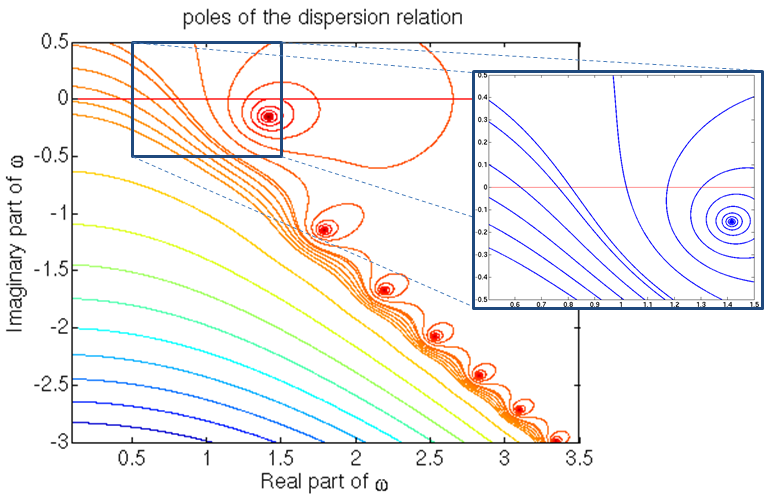
\includegraphics[width=10cm]{Figures/Fig_Landau_poles_zoom.png}
		\caption{Logarithm of the inverse of $\mathcal{D}$, eq.~\eqref{eq_VlasovPoisson_reldisp_FC}, for $k = 0.5$. The extremum gives the Landau damping: $(\omega_r,\gamma) \approx (1.41, -0.15)$.} \label{fig_Landau_DispRel}
	\end{center}
\end{figure}


\subsubsection{Physics of Landau damping}

The following analysis details the physics mechanism behind Landau damping.
Let's consider electrons immersed in a wave of the electric potential of the form $\phi = \phi_k \cos(kx-\omega t)$. Their trajectory derives from their Hamiltonian $H=mv^2/2-e\phi$:
\begin{eqnarray*}
	\dot{x}   &=& \frac{\partial H}{m\partial v} = v \\
	m \dot{v} &=& - \frac{\partial H}{\partial x} = -ek\phi_k \sin(kx-\omega t)
\end{eqnarray*} 
Let us denote $(x_0,v_0)$ the initial position and velocity of a given particle, so that:
\begin{eqnarray*}
	x(t)   &=& x_0 + v_0 t + \int_0^t \delta v(x,t^\prime)\dd t^\prime \\
	v(x,t) &=& v_0 + \delta v(x,t) 
	\;\;\; \textrm{with} \;\;\;
	\frac{\dd\, \delta v}{\dd t} = - \frac{ek\phi_k}{m} \sin(kx-\omega t)
\end{eqnarray*}
At short times $t\ll1$, one can retain the ballistic motion only $x(t) \approx x_0+v_0t$ to compute $\delta v$, so that:
\begin{equation*}
\frac{\dd\, \delta v}{\dd t} \approx - \frac{ek\phi_k}{m} \sin[k(x_0 + v_0t) -\omega t]
\end{equation*}
Now consider those particles with an initial velocity close to the phase velocity of the wave, namely $v_0 = \omega/k + \varepsilon_v$, with $|k\varepsilon_v/ \omega| \ll 1$. For the sake of simplicity, we will assume $\omega/k>0$ hereafter, without loss of generality. The particle acceleration then reads:
\begin{eqnarray*}
	\frac{\dd\, \delta v}{\dd t} &\approx& - \frac{ek\phi_k}{m} \sin(kx_0 + k\epsilon_v t) \\
	&=& - \frac{ek\phi_k}{m} [\sin(kx_0) \cos(k\epsilon_vt) + \cos(kx_0) \sin(k\epsilon_vt)]
\end{eqnarray*}
Which leads to an increment of velocity (the constant $C^{st}$ ensures that $\delta v(x,t=0)=0$, according to our hypothesis) which scales linearly with time:
\begin{eqnarray*}
	\delta v &=& - \frac{e\phi_k}{m\epsilon_v} [\sin(kx_0)\sin(k\epsilon_vt) - \cos(kx_0)\cos(k\epsilon_vt)] + C^{st}\\
	&\approx& - \frac{ek\phi_k}{m} \sin(kx_0)\; t 
\end{eqnarray*}
Whether $\delta v$ will increase or decrease with time depends on the initial phase of the particle, namely on $\sin(kx_0)$. \\

Now consider particles moving initially slightly slower than the wave, i.e. such that $\varepsilon_v<0$. Those which will be accelerated (for which $\delta v >0$) will have their velocity getting closer to the phase velocity, so that they will keep interacting with the wave a long time. Also, they will gain kinetic energy since $m(v_0+\delta_v)^2/2 > mv_0^2/2$ (remember our convention $\omega/k>0$). Conversely, those which are decelerated will move further away from the resonance, hence interacting weakly with the wave. In summary, and because energy transfer is due to resonant interactions between waves and particles, most of the energy transfer will go from the wave to these ``slow'' particles.

Performing the same analysis for particles moving slightly faster  $\varepsilon_v>0$ would lead to the opposite conclusion: most of the energy transfer goes from those ``fast'' particles to the wave.

Then, to decide whether the wave ultimately gains or looses energy, one has to count the number of particles of each category. If the equilibrium distribution function is a Maxwellian, then there are more particles slower than the wave than faster. As a result, the net balance will be in favor of the particles, and the wave will loose energy. This corresponds to Landau damping.
Conversely, if the equilibrium distribution function presents a bump on the tail characterizing an inversion of population at the phase velocity, then more energy will be transfered to the wave. Such a regime leads to the so-called ``bump-on-tail'' instability.

%===========================================
%===========================================
\section{Bump-on-tail instability} \label{sec:BoT}
%===========================================
%===========================================

The so-called ``bump-on-tail'' instability is a kinetic instability. It develops when the equilibrium distribution function presents a positive slope with respect to velocity in the tail. In particular, it can occur when a low density plasma beam of finite mean velocity interacts with the bulk plasma, at rest.

\subsection{Model for the bump-on-tail instability} 

In the following, the bump-on-tail instability is studied by means of a simple model. Let us consider the system described by eq.\eqref{eq_VlasovPoisson} (see section \ref{s_LandauDamping}).
\beqa
  && \partial_t f + v\partial_x f + \partial_x\phi \partial_v f = 0
  \label{eq_Vlasov2D} \\
  && \partial_x^2\phi = \int_{-\infty}^{+\infty}\!\! f\dd v - 1
  \label{eq_Poisson2D}
\eeqa
Conversely to section \ref{s_LandauDamping}, we consider an equilibrium made of 2 Maxwellians $f_{eq} = f_1 +f_2$ (cf. fig.~\ref{fig_BonT_Feq}): the bulk plasma particles $f_1$, at rest, of density $n_1=(1-\varepsilon)$ and temperature unity, and a beam $f_2$ of constant velocity $v_0$, of small density $n_2=\varepsilon$ and temperature $T_0$, with $\varepsilon$ a small positive parameter $0\leq \varepsilon \leq1$:
\beqa
f_1 &=& \frac{1-\varepsilon}{\sqrt{2\pi}}\; \exp\left\{ \frac{-v^2}{2}\right\}
\label{eq_f1} \\
f_2 &=& \frac{\varepsilon}{\sqrt{2\pi T_0}}\;
\exp\left\{ \frac{-(v-v_0)^2}{2T_0}\right\}
\label{eq_f2}
\eeqa
The equilibrium electric potential is vanishing: $\phi_{eq}=0$. \\

\begin{figure}[!h]
\begin{center}
  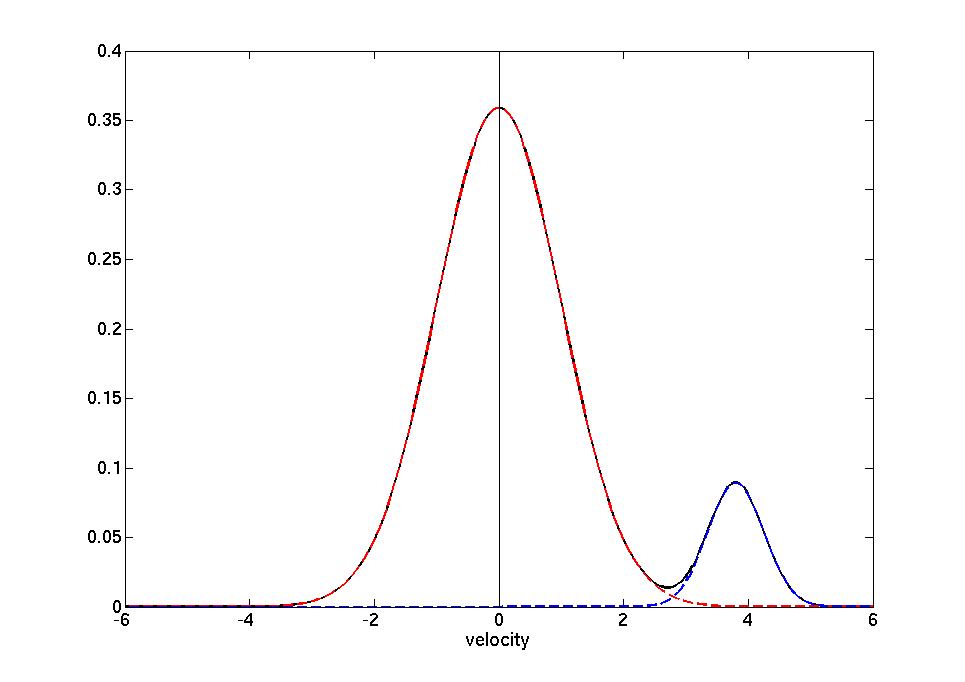
\includegraphics[width=8cm]{Figures/Fig_Feq_BoT.png}
\caption{Equilibrium distribution function $f_{eq}$. It is made of 2 Maxwellians: $f_{eq} = f_1 +f_2$.} \label{fig_BonT_Feq}
\end{center}
\end{figure}

Let us consider small amplitude fluctuations around the equilibrium given by eqs.\eqref{eq_f1}-\eqref{eq_f2}: $\tilde\phi(x,t) \ll1$ and $f=f_{eq}(v) + \tilde f(x,v,t)$, with $\tilde f\ll f_{eq}$. Following the same procedure as the one detailed in section \ref{s_LandauDamping}, one obtains the dispersion relation for harmonic fluctuations $\tilde \phi = \sum_{k,\omega} \hat \phi_{k,\omega} \exp\{i(kx-\omega t)\}$. Again, using appropriate change of variables, the dispersion relation can be expressed in terms of the plasma dispersion function:
\begin{equation}
  \label{eq_VlasovPoisson_reldisp_BoT_FC}
  \mathcal{D} (k,\omega)= k^2 
  + (1-\varepsilon)\left\{ 1 + \zeta_1 \, Z(\zeta_1) \right\} 
  + \frac{\varepsilon}{T_0}\left\{ 1 + \zeta_2 \, Z(\zeta_2) \right\} + = 0
\end{equation}
where $\zeta_1 = \omega/(\sqrt{2}|k|)$ and $\zeta_2 = (\omega-kv_0)/(\sqrt{2T_0}|k|)$. Here, $\omega \in \mathbb{C}$ stands for the complex frequency. \\

Qualitatively, unstable modes $k$ are such that their phase velocity $v_{\varphi,k} = \omega_r/k$ (with $\omega_r =\Re({\omega})$) is in the region of the positive slope $\partial_v f_{eq}$ of the total distribution function. If the beam has a small density $\varepsilon$ and in the limit of small wave vectors (large wave length with respect to the Debye length), then $\omega_r$ is roughly given by the Bohm-Gross relationship, eq.~\eqref{eq:Bohm_Gross}.

\begin{figure}[!h]
	\begin{center}
		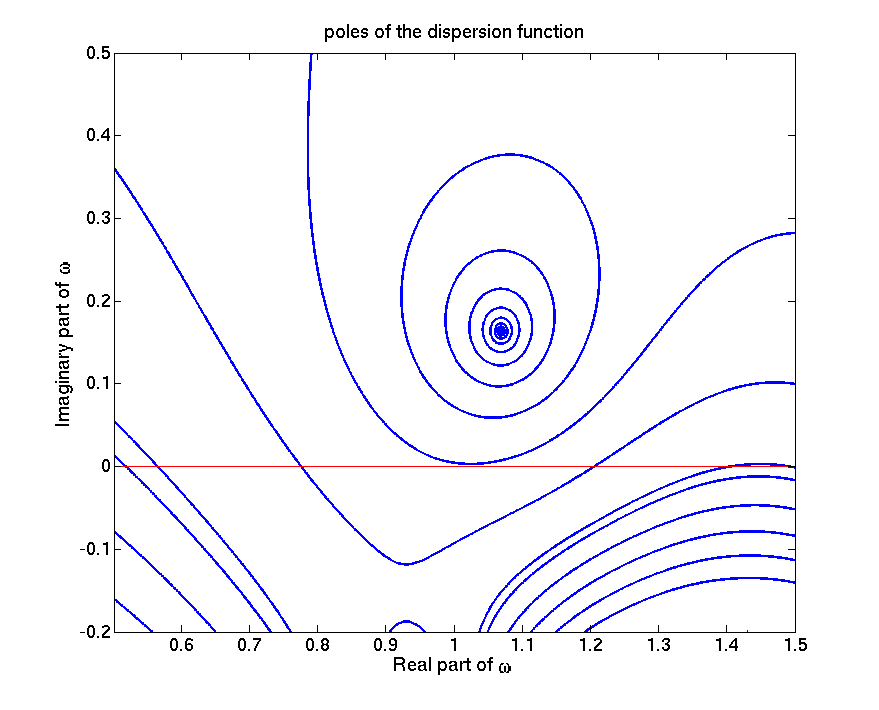
\includegraphics[width=8cm]{Figures/Fig_BoT_DispRel.png}
		\caption{Logarithm of the inverse of $\mathcal{D}$, eq.~\eqref{eq_VlasovPoisson_reldisp_BoT_FC}, for $k\approx 0.377$ and the equilibrium distribution plotted on fig.~\ref{fig_BonT_Feq}. The extremum corresponds to the unstable solution: $(\omega_r,\gamma) \approx (1.07, 0.16)$.} \label{fig_BoT_DispRel}
	\end{center}
\end{figure}

%------------------------------------------------------------------
\subsection{Resonant interaction and particle trapping}

The linear dispersion relation, eq.~\eqref{eq_VlasovPoisson_reldisp2}, shows that much physics occurs at the resonance, when particles have the resonant velocity, equal to the phase velocity $v_R=\omega/k$. We show here that, when accounting for nonlinear terms, wave-particle interaction actually also takes place in the neighborhood of the resonance: the resonance is not a Dirac centered on $v_R$, but exhibits some broadening around $v_R$. Such a physics can be addressed numerically in the frame of the bump-on-tail instability, where the exponential growth of the electric potential perturbations in the linear regime allows one to visualize the trapping of particles in the wave. \\

Let's consider the case of a single wave of given wave vector $k$ and frequency $\omega$: $\phi = \phi_k\cos(kx-\omega t)$. The resonant condition corresponds to particles having a velocity equal to the phase velocity of the wave: $v_R=\omega/k$. They are such that they see the perturbation with a constant phase $\alpha$: $\alpha_R = kx_R-\omega t=Cst$, with $\dd_t x_R=v_R$.

Close to the resonance, for particles characterized by a velocity $v=v_R+\tilde v$, with $\tilde v\ll v_R$, the Hamiltonian eq.\eqref{eq:Hamiltonian} can be Taylor expanded at first order:
\beq
H(x,v,t) \approx H(x,v_R,t) + \tilde v\; \partial_vH|_{v=v_R}
\eeq
Then, the equation of motion reads as follows:
\beqa
\dd_t x &\approx& \partial_v H|_{v=v_R} + \tilde v \; \partial^2_vH|_{v=v_R} = v_R + \tilde v \\
\dd_t v &=& \dd_t \tilde v = \partial_x\phi = - k\phi_k\; \sin(kx-\omega t)
\eeqa
Focusing on the new set of coordinates $(\alpha,\tilde v)$ instead of $(x,v)$, one readily sees that they are canonically conjugated with respect to the new Hamiltonian $K$:
\beq \label{eq:hamiltonian_K}
K\equiv k\left( \frac{\tilde v^2}{2} - \phi_k\; \cos\alpha \right)
\eeq
Indeed:
\beqa
\dd_t \alpha &=& k\, \dd_t x - \omega =k \tilde v = \partial_{\tilde v} K \\
\dd_t \tilde v &=& - k \phi_k \sin\alpha = -\partial_\alpha K
\eeqa
If $K$ does not depend explicitly on time, i.e. if $\partial_t\phi_k=0$, then it is a motion invariant. This means that the trajectories follow the iso-$K$ contours. It turns out that $K$ is analogous to the Hamiltonian of a pendulum\footnote{The Hamiltonian for a pendulum of mass unity reads $H=\frac{1}{2}\,R^2\dot{\theta}^2 -g R \cos\theta$, with $g$ and $R$ the gravity and the rotation radius, respectively. In this case, the canonical variables are the angle $\theta$ between the pendulum and the vertical axis, and the velocity $R\dot{\theta}$.}
The iso-contours of $K$ are plotted on Fig.~\ref{fig_island}. Two types of trajectories can be distinguished. From the expression of $K$, we get:
\beq
\tilde v = \pm  \sqrt{2(K/k+\phi_k\; \cos\alpha)}
\eeq
If $K>k\phi_k$, the particle trajectories are weakly affected by the wave (this corresponds to free rotation in the pendulum case). Conversely, if $K<k\phi_k$, particles are trapped in the wave and bounce back at the turning points $\alpha_0 =\arccos \{K/(k\phi_k)\}$ (so-called libration motion for the pendulum). The separatrix corresponds to the special case $K=k\phi_k$. Its width at the O-point scales like the square-root of the magnitude of the perturbation:
\beq
\delta \tilde v_{sep.} = 4\; \sqrt{\phi_k}
\eeq
These are those particles trapped in the wave that most interact with it. $\delta \tilde v_{sep.}$ measures the broadening of the resonance.


\begin{figure}[!h]
	\begin{center}
		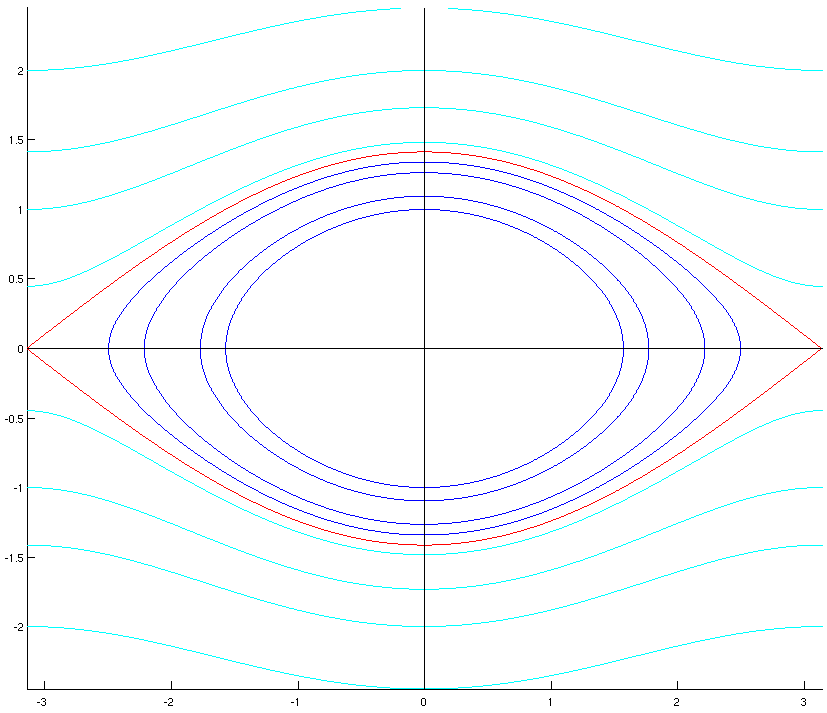
\includegraphics[width=6cm]{Figures/Fig_island.png}
		\caption{Iso-contours of the Hamiltonian $K$ (cf. eq.\eqref{eq:hamiltonian_K}). The $x$ and $y$ axis are respectively $\alpha$ and $\tilde v$. $\tilde v=0$ corresponds to the resonance condition, $v=v_R$.} \label{fig_island}
	\end{center}
\end{figure}


%===========================================
\newpage
%\vspace{5cm}
\appendix
%===========================================
\section{Mathematical developments for Landau damping}
\label{Appendix_Landau}

\subsection{Analytic continuation issue}

Let's consider the following integral:
\begin{equation}
  I \equiv \int_{-\infty}^{\infty} \frac{g(x)}{x-x_0}\; \dd x
\end{equation}
where $g(x)$ is some continuous and derivable function on $\mathbb{R}$, and $x_0$ some real constant. Such an integral \emph{a priori} diverges due to the presence of the pole -- or resonance -- for $x=x_0$. The analytic continuation consists in slightly modifying the integration contour so that the integral remains well defined, while still retaining the effect of the pole. The trick is to immerge the integrant in the complex plane $z\in \mathbb{C}$, with $x=\Re(z)$, so that the contour goes from $-\infty$ to $+\infty$ on the real axis, except at the very location of the pole which is encircled, as illustrated on fig.\ref{fig_Landau}. From the mathematical point of view, two contours can be equally chosen arbitrarily, namely $D_+$ or $D_-$ (see the red contours on fig.\ref{fig_Landau}). The magnitude of the radius $\epsilon>0$ of the semi-circles which circumscribe the pole $x_0$ tends to zero. However, as we will show, they lead to two different expressions for the integral $I$:
\begin{eqnarray*}
 I_{\pm} &\equiv& \int_{D_\pm} \frac{g(z)}{z-x_0}\; \dd z \\
   &=&
   \lim_{\epsilon\to0} \left\{
   \int_{-\infty}^{x_0-\epsilon} \frac{g(x)}{x-x_0}\; \dd x +
   \int_{x_0+\epsilon}^\infty \frac{g(x)}{x-x_0}\; \dd x
   \mp \int_0^{\pi} \frac{g(x_0+\epsilon\ee^{i\theta})}{x_0+\epsilon\ee^{i\theta}-x_0}\;
   i\epsilon\ee^{i\theta}\dd \theta \right\}
\end{eqnarray*}
The first two terms are nothing else but the principal part of the integral, which we shall denote $\mathsf{P}\!\int$ hereafter. The last term can be recast as follows (notice that the limit $\epsilon\to0$ commutes with the integral):
\begin{eqnarray*}
 \lim_{\epsilon\to0} \int_0^{\pi} i\, g(x_0+\epsilon\ee^{i\theta}) \dd \theta
   = i\pi\; g(x_0)
\end{eqnarray*}
Finally, the integrals $I_\pm$ are given by:
\begin{equation}
 I_{\pm} \equiv \int_{D_\pm} \frac{g(z)}{z-x_0}\; \dd z
 = \mathsf{P}\!\int_{-\infty}^{\infty} \frac{g(x)}{x-x_0}\; \dd x
       \mp i\pi\, g(x) \,\delta(x-x_0)
\end{equation}
It appears that the sign of the imaginary part depends on the contour $D_-$ or $D_+$ chosen to circumscribe the pole.


\subsection{Alternative expressions of the integrals $I_\pm$}

Cauchy's theorem for holomorphic functions provides a way to find equivalent expressions of an integral with different contour paths. Let us first recall the definition of {\bf holomorphic functions}:
\begin{quote}
 A holomorphic function is a complex-valued function of one or more complex variables that is complex-differentiable in a neighborhood of every point in its domain\footnote{We recall that the complex-derivative of any function of a complex argument is defined as: $\dd F(z)/\dd z \equiv \lim_{|h|
\rightarrow 0} \{F(z_0+h)-F(z_0)\}/|h|$, with $h\in \mathbb{C}$.
Notice especially that the derivative at $z_0$ should not depend on the
direction one approaches $z_0$ in the complex plane.}. The existence of a complex derivative is a very strong condition, for it can be shown that it implies that any holomorphic function is actually infinitely differentiable and equal to its own Taylor series. Put differently, the class of \emph{holomorphic functions} coincides with the class of \emph{complex analytic functions}, which constitutes one of the major theorems in complex analysis.
\end{quote}
{\bf Cauchy's theorem} then states:
\begin{quote}
 If $F(z)$ is holomorphic within and on the closed contour $\mathcal{C}$ in the complex plane, then $\int_\mathcal{C} F(z) \dd z=0$.
\end{quote}
Conversely, the Residue theorem applies for non analytic functions. Especially:
\begin{quote}
 If $F(z)$ has $N$ singularities $z_j$ within $\mathcal{C}$, then $\int_\mathcal{C} F(z) \dd  z= 2i\pi \sum_{j=1}^N $ $\textrm{Res}\{F(z_j)\}$, where Res$\{F(z_j)\}$ denotes the residue at $z_j$. Here is estimated the impact of encircling the pole when deforming the contour.
\end{quote}

\begin{figure}[htbp]
  \begin{center}
  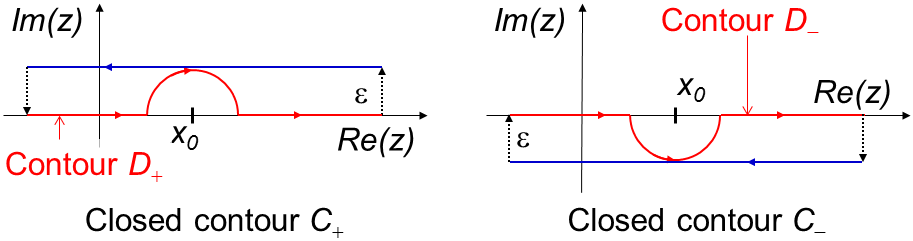
\includegraphics[width=14cm]{Figures/Fig_contourLandau.png}
  \end{center}
\caption{Contours of integration used in eq.\eqref{eq:equiv_Cauchy}.}
 \label{fig_Landau}
\end{figure}

Cauchy's theorem allows one to recast the integrals $I_\pm$. First notice that $F(z) \equiv g(z)/(z-x_0)$ is holomorphic on and within the closed contours $\mathcal{C}_\pm$ drawn on fig.\ref{fig_Landau}. Indeed, such contours do explicitly exclude the pole $x_0$. Therefore, $\int_{\mathcal{C}_\pm} F(z)\dd z=0$ in virtue of Cauchy's theorem. Notice then that the closed contours $\mathcal{C}_\pm$ contain the open contours $D_\pm$. More precisely:
\begin{eqnarray}
 \int_{\mathcal{C}{\pm}} \frac{g(z)}{z-x_0}\; \dd z &=& 0 \nonumber\\
 &=&\lim_{\epsilon\to0^+} \left\{
 \lim_{R\to+\infty}\left(
 \int_0^{\pm\epsilon} \frac{g(R\pm i\zeta)}{R\pm i\zeta-x_0}\; i\dd \zeta +
 \int_{\pm\epsilon}^0 \frac{g(-R\pm i\zeta)}{-R\pm i\zeta-x_0}\; i\dd \zeta \right)\right.
 \nonumber \\
 &&\left. + \int_{+\infty}^{-\infty} \frac{g(x\pm i\epsilon)}{x\pm i\epsilon-x_0}\; \dd x + \int_{D_\pm} \frac{g(z)}{z-x_0}\; \dd z \right\}
 \label{eq:equiv_Cauchy}
\end{eqnarray}
It is easy to show that the first two integrals vanish. Indeed, Taylor expanding both $g$ and the denominator in the limit $\zeta/R\to0$ or $\zeta/(R\pm x_0)\to0$\footnote{One can indeed expand the denominator in this case since $R$ tends to infinity. Therefore, there is no pole or resonance, even for $\zeta=0$.} shows that each term of the series vanishes when integrating $\zeta$ from 0 to $\epsilon$, with $\epsilon\to0$ (remember that $g$ is analytic and bounded). Then, it follows that the last two terms cancel each other. Finally, due to the analyticity of $g$, $g(x\pm i\epsilon)$ can be replaced by $g(x)$ in the limit $\epsilon\to0$ in the third integral on the right hand side, such that, ultimately:
\begin{equation}
  I_\pm \equiv \int_{D_\pm} \frac{g(z)}{z-x_0}\; \dd z
  = \int_{-\infty}^{+\infty} \frac{g(x)}{x-x_0\pm i\epsilon}\; \dd x
\end{equation}


\subsection{The plasma dispersion function $Z(\zeta)$}

The plasma dispersion function, also known as the Fried and Conte function \footnote{B.D. Fried and S.D. Conte, The Plasma Dispersion Function (Academic Press, New York NY, 1961)}, is defined in the whole complex plane $\zeta\in\mathbb{C}$ by:
\begin{eqnarray}
 Z(\zeta) &=& \frac{1}{\sqrt{\pi}}\int_{-\infty}^{+\infty} \frac{\ee^{-x^2}}{x-\zeta}\; \dd x \;\;\;\;\;\;\;\;\;\;\;\;\;\;\;\;\;\;\;\;\;\;\;\;\;\; \textrm{if }\zeta_i>0
 \label{eq:Zeta_1}\\
 &=&\frac{1}{\sqrt{\pi}}\int_{-\infty}^{+\infty} \frac{\ee^{-x^2}}{x-\zeta}\; \dd x + 2i\sqrt{\pi}\; \ee^{-\zeta^2}\;\;\;\;\;\;\, \textrm{if }\zeta_i<0 \label{eq:Zeta_2}\\
 &=&\frac{1}{\sqrt{\pi}}\;\mathsf{P}\!\!\!\int_{-\infty}^{+\infty} \frac{\ee^{-x^2}}{x-\zeta}\; \dd x + i\sqrt{\pi}\; \ee^{-\zeta^2}\;\;\;\;\;\;\; \textrm{if }\zeta_i=0 \label{eq:Zeta_3}
\end{eqnarray}
The three cases correspond to the three contours illustrated on fig.\ref{fig_contourZ}.

\begin{figure}[htbp]
  \begin{center}
  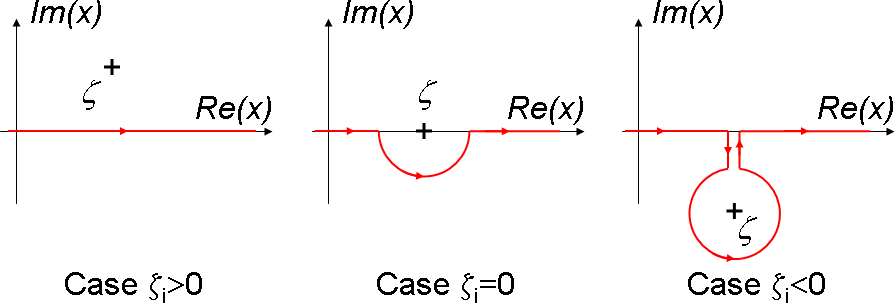
\includegraphics[width=14cm]{Figures/Fig_contourZ.png}
  \end{center}
\caption{Contours of integration corresponding to the three cases eqs.(\ref{eq:Zeta_1}-\ref{eq:Zeta_3}).}
 \label{fig_contourZ}
\end{figure}
For small magnitudes of the argument $|\zeta|\ll1$, $Z(\zeta)$ can be expanded as follows:
\beq
  Z(\zeta) \approx i\pi^{1/2}\ee^{-\zeta^2} -
  2\zeta\left[ 1 - \frac{2}{3}\,\zeta^2 + \frac{4}{15}\,\zeta^4 + ...\right]
\eeq

%===========================================
\section{Wave-particle energy transfer}
\label{Appendix_Wint}

The energy carried by electromagnetic waves reads as follows:
\begin{equation}
  \mathcal{E}_{EM} = \frac{1}{2}\;
  \int \dd V\left( \frac{B^2}{\mu_0} + \epsilon_0 E^2\right)
\end{equation}
with $E$ and $B$ the electric and magnetic field intensity, respectively. Using Maxwell's relations:
\begin{eqnarray*}
  \nablabf \times \Ebf &=& -\partial_t \Bbf \\
  \nablabf \times \Bbf &=& \mu_0 \jbf +
  \frac{1}{c^2}\partial_t \Ebf
\end{eqnarray*}
with $\epsilon_0 \mu_0 c^2=1$, one can compute the time evolution of $\mathcal{E}_{EM}$:
\begin{eqnarray*}
  \mathcal{P}_{EM} \equiv \frac{\partial \mathcal{E}_{EM}}{\partial t}
  &=& \int_V \dd V \left( \frac{\Bbf}{\mu_0}.\; \partial_t\Bbf+
  \epsilon_0 \Ebf. \partial_t\Ebf\right) \\
  &=& \int_V \dd V \left( \frac{\Ebf.(\nablabf \times\Bbf)-
  \Bbf.(\nablabf \times\Ebf)}{\mu_0} -\Ebf.\jbf\right)\\
  &=& -\int_V \dd V\; \nablabf.\left(\frac{\Ebf\times\Bbf}{\mu_0}\right)
  -\int_V\dd V\; \Ebf.\jbf
\end{eqnarray*}
Then, using Ostrogradsky's formula $\int \dd V\; \nablabf.\Fbf =\int \dd \Sbf.\Fbf$, it reads:
\begin{equation}
  \mathcal{P}_{EM} = - \int_S \dd \Sbf.\; \frac{\Ebf\times \Bbf}{\mu_0} -
  \int_V\dd V\; \Ebf.\jbf
\end{equation}
The first term is the integral of the Poynting vector over the closed surface encircling the considered system. It accounts for energy exchanges with the exterior. The second term accounts for the wave-particle energy transfer within the volume of the system. Using the charge conservation equation $\partial_t \rho + \nablabf.\jbf=0$ (with $\rho$ the charge density), one obtains after an integration by part:
\begin{eqnarray*}
  P_{EM} &\equiv& -\int_V\dd V\; \Ebf.\jbf \\
  &=& \int_V \dd V\; \left(\phi \;\partial_t \rho +
  \jbf. \partial_t\Abf \right)
\end{eqnarray*}
with $\Abf$ the vector potential: $\Bbf=\nablabf \times \Abf$ and $\Ebf =-\nablabf \phi-\partial_t \Abf$.\\

Let us consider the case of an electrostatic wave $\tilde\phi$ of real frequency $\omega$: $\tilde\phi = \phi$e$^{-i\omega t}+\phi^*$e$^{i\omega t}$. The power density $p_{EM}$ transferred by the particles to the wave is given by:
\begin{eqnarray*}
  p_{EM} = \tilde\phi \;\partial_t \tilde\rho
  &=& -i\omega\;
  \left( \phi \textrm{e}^{-i\omega t}+\phi^*\textrm{e}^{i\omega t} \right)
  \left( \rho \textrm{e}^{-i\omega t}-\rho^*\textrm{e}^{i\omega t}
  \right)\\
  &=& 2\omega\;\textrm{Im}
  \left( \rho\phi \textrm{e}^{-2i\omega t}+\rho\phi^*\right)
\end{eqnarray*}
The oscillatory first term does not contribute to any transfer on long time durations (larger than $\omega^{-1}$). The final result is then that the power density transferred from particles to an electrostatic wave of frequency $\omega$, reads as follows:
\begin{equation}
  p_{EM} = 2\omega\;\textrm{Im} (\rho\phi^*)
\end{equation}


%===========================================
\section{Analytic expression of Landau damping in a limit case}
\label{Appendix_gamma_Landau}

Let us assume that complex frequencies $\omega=\omega_r+
i\omega_i$, such that $\omega_i \ll \omega_r$, are solutions of
the dispersion relation eq.\eqref{eq_VlasovPoisson_reldisp2}. The ordering between the real and imaginary parts can be verified \emph{a posteriori}. In this
case, $\mathcal{D}(k,\omega)$ can then be Taylor expanded as a
function of this small parameter. At first order, and denoting
$\mathcal{D} = \mathcal{D}_r + i\mathcal{D}_i$, this leads to:
\begin{equation*}
\mathcal{D}(k,\omega) \approx
\mathcal{D}_r(k,\omega_r)
- \omega_i \left.
\frac{\partial \mathcal{D}_i(k,\omega)}{\partial \omega}\right|_{\omega_r}
+ i\left\{\mathcal{D}_i(k,\omega_r)
+ \omega_i \left.
\frac{\partial \mathcal{D}_r(k,\omega)}{\partial \omega}
\right|_{\omega_r}\right\} =0
\end{equation*}
Besides, the imaginary part of the dispersion relation
$\mathcal{D}_i$ is smaller than the real part $\mathcal{D}_r$.
Taking the limit $\mathcal{D}_i \ll \mathcal{D}_r$, the previous
equation reduces to:
\begin{eqnarray*}
	&& \omega_i = -\frac{\mathcal{D}_i(k,\omega)}
	{\;\left.\partial_\omega\mathcal{D}_r(k,\omega)\right|_{\omega_r}} \\
	&& \mathcal{D}_r(k,\omega_r) = 0
\end{eqnarray*}
The imaginary part $\omega_i$ turns out to vanish in the absence of the imaginary part of the
dispersion relation $\mathcal{D}_i$, namely of the resonance
condition. Let us consider the case of a Maxwellian equilibrium:
\beq \label{eq:feq_Maxwell}
f_{eq} = \frac{1}{\sqrt{2\pi}}\; \ee^{-v^2/2}
\eeq
In this case, the imaginary part is simply:
\beq
\mathcal{D}_i(k,\omega_r)
= \sqrt{\frac{\pi}{2}}\; \frac{\omega_r}{|k|}\; \ee^{-\omega_r^2/2k^2}
\eeq
The real frequency $\omega_r$ can be estimated in the hydrodynamical limit $\omega_r\gg kv$, by Taylor expanding the denominator of the integrand present in $\mathcal{D}_r$. Up to $4^{th}$ order, it reads as follows:
\beqas
\mathcal{D}_r(k,\omega_r) &=&
k^2 - \textsf{P} \int_{-\infty}^{+\infty}
\frac{kv\; \ee^{-v^2/2}}{\omega_r(1-kv/\omega_r)} \,\frac{\dd v}{\sqrt{2\pi}} \\
&\approx& k^2 -  \int_{-\infty}^{+\infty} \frac{kv\; \ee^{-v^2/2}}{\omega_r}
\left\{\frac{kv}{\omega_r} + \left(\frac{kv}{\omega_r}\right)^3 \right\} \,\frac{\dd v}{\sqrt{2\pi}} \\
&\approx& k^2 -  \frac{k^2}{\omega_r^2} - \frac{3k^4}{\omega_r^4} = 0
\eeqas
In the limit of small wave vectors $k\ll 1$, corresponding to large wavelength as compared to Debye length, the solution is given by the Bohm-Gross\footnote{D. Bohm and E. P. Gross, ``Theory of Plasma Oscillations. A. Origin of Medium-Like Behavior'', \emph{Phys. Rev.} {\bf 75} (1949) 1851} relationship:
\beq
\label{eq:Bohm_Gross}
\omega_r^2 \approx 1 + 3 k^2
\eeq
These are the so-called \emph{Langmuir waves}. In true units, they read: $\omega_r^2 = \omega_p^2 (1+3k^2\lambda_D^2)$. \\

Considering the same limit to derive the expression of the imaginary part $\gamma_L \equiv \omega_i$, one readily finds that $\left.\partial_\omega\mathcal{D}_r(k,\omega)\right|_{\omega_r} = 2k^2$ at lowest order (i.e. taking $\omega_r=1$). $\gamma_L$ then becomes:
%\begin{equation} \label{eq_gammaL}
%  \gamma_L = -\sqrt{\frac{\pi}{2}}\; \frac{\omega_r}{k|k|} \;
%  \exp\left\{-\frac{1}{2} \left(\frac{\omega_r}{k} \right)^2 \right\}
%  \;\frac{1}{\textsf{P}\int_{-\infty}^{+\infty}\! \frac{v\textrm{e}^{-v^2/2}}
%  {(\omega_r - kv)^2} \,\dd v}
%\end{equation}
\beq
\gamma_L = - \sqrt{\frac{\pi}{8}}\; \frac{1}{|k|^3}\; \ee^{-1/2k^2}
\eeq
or $\gamma_L = - \sqrt{\pi/8}\; \omega_p\; |k\lambda_D|^{-3}\; \exp\left[ -1/2(k\lambda_D)^2 \right]$ in true units. It turns out that $\gamma_L$ is always negative. It is
known as the \emph{Landau damping}. Waves are damped away by transferring
energy to the particles. Since its first derivation in 1946, Landau damping has been the object of much discussion, aiming at understanding the 'paradox' of an apparently irreversible process (the damping of the injected wave) being predicted by a collisionless $-$ hence reversible $-$ model, namely Vlasov equation. Actually, the wave damping is not a dissipative process: the energy is transferred to the particles, and the whole process occurs at constant entropy. Even after the experimental confirmation of the effect in 1964\footnote{ J.H. Malmberg, C.B. Wharton, \emph{"Collisionless damping of electrostatic plasma waves", Phys. Rev. Lett.} {\bf 13} (1964) 184}, the discussion went on, and is still far from damped away\footnote{ see e.g.: DD. Ryutov, \emph{"Landau damping: half a century with the great discovery", Plasma Phys. Contr. Fusion} {\bf 41} (1999) A1-12}. \\

It is easy to show that such a resonant wave-particle interaction leads to wave damping by transferring energy to the particles. Let us evaluate the electromagnetic power density $P_{EM}$ exchanged between a wave of real frequency $\omega$ and an assembly of particles of charge density $\hat \rho_{k,\omega}$. In the present case, $\hat \rho_{k,\omega} = -\int \hat f_{k,\omega}\dd v$ for electrons. As shown in appendix~\ref{Appendix_Wint}, $P_{EM}$ reads as follows:
\beqas
P_{EM} &=& 2\omega \Im\left(\hat \rho_{k,\omega}
\hat\phi_{k,\omega}^* \right) \\
&=& 2\omega\; \Im\left\{ \int_{-\infty}^{+\infty}
\frac{kv\, \ee^{-v^2/2}}{\omega-kv}
\; \frac{\dd v}{\sqrt{2\pi}}\; |\hat \phi_{k,\omega}|^2 \right\} \\
&=& -2\omega \; |\hat \phi_{k,\omega}|^2\; \int_{-\infty}^{+\infty}
kv\, \ee^{-v^2/2}\; \pi\delta(\omega-kv) \; \frac{\dd v}{\sqrt{2\pi}} \\
&=& -\sqrt{2\pi}\; |\hat \phi_{k,\omega}|^2\; \frac{\omega^2}{|k|}
\exp\left(-\frac{\omega^2}{2k^2}\right)
\eeqas
which is always negative.

%===========================================
\end{document}
